% !TeX spellcheck = <none>
\documentclass[a4paper, 10pt]{scrartcl}  

\usepackage[width=17.00cm, height=25.00cm]{geometry}
\geometry{verbose,a4paper,tmargin=20mm,bmargin=20mm,lmargin=20mm,rmargin=20mm}

\usepackage[english]{babel}
\usepackage[utf8]{inputenc}
\usepackage{tgcursor}

\usepackage{amsmath,amssymb,amstext}
\usepackage{tikz}
\usepackage{listings}
\usepackage{graphicx}
\usepackage{scrextend}
\usepackage[colorlinks, 				% Inhaltsverzeichnis verlinken
			pdfpagelabels,
			pdfstartview = FitH,
			bookmarksopen = true,
			bookmarksnumbered = true,
			linkcolor = blue!40!black,
			plainpages = false,
			hypertexnames = false,
			citecolor = black] {hyperref}
\usepackage{array}
\usepackage{tcolorbox}
\usepackage{trfsigns}
\usepackage{transparent}
%\usepackage{eso-pic}

\setcounter{tocdepth}{3}  
\setlength{\arrayrulewidth}{0.1pt}
\setlength{\parindent}{0pt}

% Umrahmung definieren
\tcbset{fonttitle=\bfseries, colback=black!1!,colframe=green!50!black!40!}

\begin{document}
	\begin{titlepage}
%		\AddToShipoutPicture*{\put(-150,-80){\parbox[b][\paperheight]{\paperwidth}{\vfill\centering{\transparent{0.01}
\includegraphics[width=1.7\paperwidth,height=1.7\paperheight,keepaspectratio]{./pics/unilog.jpg}}\vfill	}}}
%		\ClearShipoutPicture
		\center 		
		\textsc{\huge \bfseries Berechnung Wärmeübergangskoeffizient und thermischer Widerstand aus Messdaten}\\[1cm] 
		\textsc{\Large Documentation}\\[0.5cm] 
		\textsc{\large Author: Bernd Heufelder}\\[0.5cm] 
		{\large \today}\\[1cm] 
		
\includegraphics[width=0.3\linewidth]{./pics/BesiLogo.jpg}\\[1cm]
		\begin{flushleft}
			\tableofcontents
		\end{flushleft}
	\end{titlepage}
		
	\section{Herleitung der Formel für den Wärmeübergangskoeffizient}
		Wärmeleistung nach dem Fourier'schen Gesetz
		\[\dot{Q} = \underbrace{\dfrac{\lambda}{d}}_{h}\cdot A\cdot (T(t) - T_{\infty}) \]
		\begin{tabbing}
			$ \lambda $ \= ... \= Wärmeleitungskoeffizient in $ [k\frac{W}{m\cdot K}] $\\	
			$ d $ \> ... \> Materialstärke in $ [m] $\\	
			$ h $ \> ... \> Wärmeübergangskoeffizienten in $ [\frac{W}{m^{2}\cdot K}] $\\
			$ A $ \> ... \> an der Wärmeübertragung beteiligte Fläche $ [m^{2}] $\\
		\end{tabbing}
		Für die Energiebilanz gilt:
		\[\dot{Q} = m\cdot c\cdot \dfrac{dT(t)}{dt}\]
		Durch Gleichsetzen ergibt sich die folgende inhomogene lineare DGL 1. Ordnung
		\[h\cdot A\cdot (T(t) - T_{\infty}) =  m\cdot c\cdot \dfrac{dT(t)}{dt}\]
		Die Lösung dieser DGL ist durch
		\[T(t) - T_{\infty} = (T_{0}-T_{\infty})\cdot e^{-\frac{h\cdot A}{m\cdot c}\cdot t}\]
		gegeben. Umformen nach dem Wärmeübergangskoeffizienten $ h $ ergibt 
		\begin{tcolorbox}[title=Wärmeübergangskoeffizienten $ h $]
			\[h = -ln\bigg(\dfrac{T(t) - T_{\infty}}{T_{0}-T_{\infty}}\bigg)\cdot \dfrac{m\cdot c}{t\cdot A}  \qquad \text{in } \bigg[\frac{W}{m^{2}\cdot K}\bigg]\]
			\tcblower
			\begin{tabbing}
				$ m $ \= ... \= Masse in $ [kg] $\\	
				$ c $ \> ... \> spezifische Wärmekapazität in $ [\frac{J}{K\cdot kg}] $\\	
				$ A $ \> ... \> am Wärmetransport beteiligte Fläche in $ [m^{2}] $\\
				$ T_{\infty} $ \> ... \> Umgebungstemperatur in $ [^{\circ}C] $\\
			\end{tabbing}
			
		\end{tcolorbox}	
		\begin{figure}[h!]
			\centering
			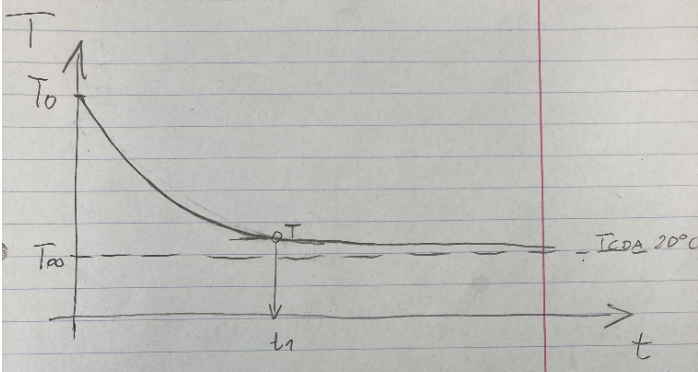
\includegraphics[width=0.8\linewidth]{./pics/coolcurve.png}
			\caption{Skizze einer typischen Abkühlkurve (PT1-Verhalten)}
		\end{figure}
		
		Anhand dieser Formel kann nun aus einer gemessenen Abkühlkurve der Wärmeübergangskoeffizient in $ \frac{W}{m^{2}\cdot K} $ berechnet werden. 
	\section{Thermischer Widerstand}
		Der thermische Widerstand gibt an welcher Wärmestrom sich bei einer gewissen Temperaturdifferenz $ \Delta T $ einstellt. Z.b. kann damit der Wärmestrom zwischen einem heißen Objekt und seiner Umgebung berechnet werden, wenn die Temperaturdifferenz bekannt ist. Es ist demnach ein Absolutwert und nicht auf eine spezifische Fläche bezogen.
		\begin{tcolorbox}[title=Definition des Wärmewiderstands]
			\[ R_{th} = \dfrac{\Delta T}{\dot{Q}} \qquad \text{in } \bigg[\frac{K}{W}\bigg]\]	
			\tcblower
			\begin{tabbing}
				$ \Delta T $ \= ... \= Temperaturdifferenz, z.b. zwischen einer Kühloberfläche und der Umgebung in $ [K] $\\	
				$ \dot{Q} $ \> ... \> Wärmestrom, z.b. von einer Kühloberfläche an seine Umgebung in $ [W] $\\	
			\end{tabbing}
			
		\end{tcolorbox}	
	
		Möchte man einen nicht-flächenbezogenen Wert für das Abkühlverhalten, dann kann dafür der thermische Widerstand herangezogen werden. Die Verknüpfung zum Wärmeübergangskoeffizienten $ h $ ist folgendermaßen gegeben:
		\begin{tcolorbox}[title=Bezug von thermischen Widerstand zum Wärmeübergangskoeffizienten]
			\[ R_{th} = \dfrac{1}{h\cdot A} \qquad \text{in } \bigg[\frac{K}{W}\bigg]\]			
		\end{tcolorbox}	
		
\end{document}